\documentclass{article}

% Language setting
% Replace `english' with e.g. `spanish' to change the document language
\usepackage{biblatex} %Imports biblatex package
\addbibresource{../Lab2/refs.bib}
\usepackage{enumitem}
\usepackage[english]{babel}
\usepackage{array}
\usepackage{amsmath}
\usepackage{pythonhighlight}
\usepackage{multirow}
\newcolumntype{P}[1]{>{\centering\arraybackslash}p{#1}}
\newcolumntype{M}[1]{>{\centering\arraybackslash}m{#1}}

% Set page size and margins
% Replace `letterpaper' with `a4paper' for UK/EU standard size
\usepackage[letterpaper,top=2cm,bottom=2cm,left=3cm,right=3cm,marginparwidth=1.75cm]{geometry}

\usepackage{amsmath}
\usepackage{graphicx}
\usepackage{caption}
\usepackage{subcaption}
\usepackage[colorlinks=true, allcolors=blue]{hyperref}
\usepackage{setspace}
\usepackage{booktabs}
\usepackage[T1]{fontenc}
\usepackage{longtable}
\doublespacing

\begin{document}
\newcommand{\Fig}[3]{\begin{figure}[!h!]\centering\includegraphics[width=0.5\linewidth]{#1}\caption{#2}\label{#3}\end{figure}}
\begin{titlepage}

\centering
\scshape
\vspace{\baselineskip}

%
\rule{\textwidth}{1.6pt}\vspace*{-\baselineskip}\vspace*{2pt}
\rule{\textwidth}{0.4pt}

{\Huge \textbf{\textsc{ Heat Treatment of Steels \\
\vspace{15pt}}}}

\rule{\textwidth}{0.4pt}\vspace*{-\baselineskip}\vspace{3.2pt}
\rule{\textwidth}{1.6pt}\vspace{6pt}
\centerline{\textit{University of Illinois at Urbana-Champaign}} 
\centerline{\textit{Department of Nuclear, Plasma, and Radiological Engineering}}
\vspace{1.5\baselineskip}


\large \centerline{\textbf{Author:} Nathan Glaser}
\large \centerline{\textbf{Net-ID:} nglaser3}
\quad

\vfill
\large \centerline{October 23, 2024}
%
\pagenumbering{gobble}
\end{titlepage}

\tableofcontents
\newpage
\pagenumbering{arabic}

\section{Abstract}
Heat treatment is a necessary portion of material casting, and the methodology chosen can have strong impacts on the resulting material properties. Specifically in Steel, small deviations in cooling time can have drastic changes on the resulting microstructure. We investigated the affects of heat treatment on resulting material properties of 4340 Steel. We measured the stress-strain curves of specimens that underwent 6 different heat treatments: Standard Oil Quenched, Standard Water Quenched, Annealed, Normalized, Oil Quenched then Tempered at 300 $^oC$, and Oil Quenched then Tempered at 500 $^oC$. From these stress-strain curves we determined the elastic modulus, the yield strength, the ultimate tensile strength, the toughness, and the percent elongation; and proximally found the Brinnel hardness of each sample. Further, we investigated the correlation between a materials ultimate tensile strength, yield strength, elastic modulus, or the percent elongation to the Brinnel hardness of each specimen. We found there is a strong dependence of material properties on heat treatment method utilized, often yielding drastically different properties. We found quicker cooling treatments yielded stronger materials that were more brittle, and slower treatments or treatments that were held at an elevated temperature to have much more ductility at the cost of a lower strength. Finally, we identified the causality for the difference between material properties to be the specific phase of the microstructures in the specimens, where martensite lead to poor ductility and spherodite and pearlite lead to more ductility.

\section{Introduction}
4340 Steel is one of the most commonly applicable materials in structural applications. 4340 Steel is composed of Iron, Chromium, and Carbon, and thus can have interesting material property dependence on heat treatment methodology in casting. Heat treatment methodology employed has a strong impact on resulting material properties, as the method used ultimately governs the rate of grain growth and ultimate dislocation density.
\newpage
\section{Experimental Methods}
To obtain our experimental results we utilized the following methodology, appropriated from \cite{manual}. The methodology for all specimens were identical, and so the procedure described is undertaken for each specimen if not explicitly specified. We tested six total specimens: Standard Oil Quenched, Standard Water Quenched, Annealed, Normalized, Oil Quenched then Tempered at 300 $^oC$, and Oil Quenched then Tempered at 500 $^oC$. 

To begin the experiment, the specimens were in a hot furnace. The specimens were then removed from the furnace and underwent their respective heat treatment:
\begin{itemize}
     \item Standard Oil Quenched --- Dunked in oil 
     \item Standard Water Quenched --- Dunked in water
     \item Annealed --- Not done by us
     \item Normalized --- Not done by us 
     \item Oil Quenched then Tempered at 300 $^oC$ --- Dunked in oil then held at 300 $^oC$
     \item Oil Quenched then Tempered at 500 $^oC$ --- Dunked in oil then held at 500 $^oC$
\end{itemize}

Next, each specimen was cleaned and then polished to remove external impurities. We measured the initial diameter of the gage, and the hardness of the grip. Then each specimen was loaded into the Tensile Tester, and a trial was ran. To run each trial we loaded the specimen, got the force to be less than 0.5 $MPa$, and then zeroed the strain. After fracture, we measured the resulting gage diameter. 

\newpage
\section{Theoretical Models}
To begin, we measured the force applied to a specimen and the resulting strain. To convert these force values to stress, we utilized the following equation:

\begin{equation}
    \sigma_e = \frac{F}{A_{xs,o}} = \frac{F}{\pi r_{o}^2}
\end{equation}
where $A_{xs,o}$ and $r_o$ are the initial cross sectional area and the initial radius of the load bearing section of the specimen, respectively. 

Next, to determine the toughness of a specimen we integrate the stress-strain curve from the yield point to the fracture point with respect to the strain. To perform the integration we utilized the numerical integrator provided by \texttt{numpy}, \texttt{numpy.trapezoid}. 
\begin{equation}
    T = \int_{\epsilon_{y}}^{\epsilon_{f}}\sigma_e\left(\epsilon\right)\ d\epsilon
\end{equation}

Next, because our measured strain values are in mm/mm units, we simply convert these to percent by multiplying by 100, and then we utilize the following equation to determine the percent elongation of the specimen.
\begin{equation}
    \%_{e} = \epsilon_{\%,f} -\epsilon_{\%,o}
\end{equation}

Finally, we measured the hardness utilizing the Rockwell C scale, however we want these reported in terms of the Brinnel scale. To convert from HRC to BHN we utilized the following theoretical equation, \cite{manual}.
\begin{equation}
    \textbf{H}_{BN} = 131.7 e^{0.0252\:\textbf{H}_{RC}}
    \label{eq:rc2br}
\end{equation}

\newpage
\section{Results}
To begin, we found the engineering stress-strain curves for oil quenched, water quenched, normalized, annealed, and oil quenched and tempered at both 300 and 500 $^oC$. 

\begin{figure}[!h!]
    \centering
    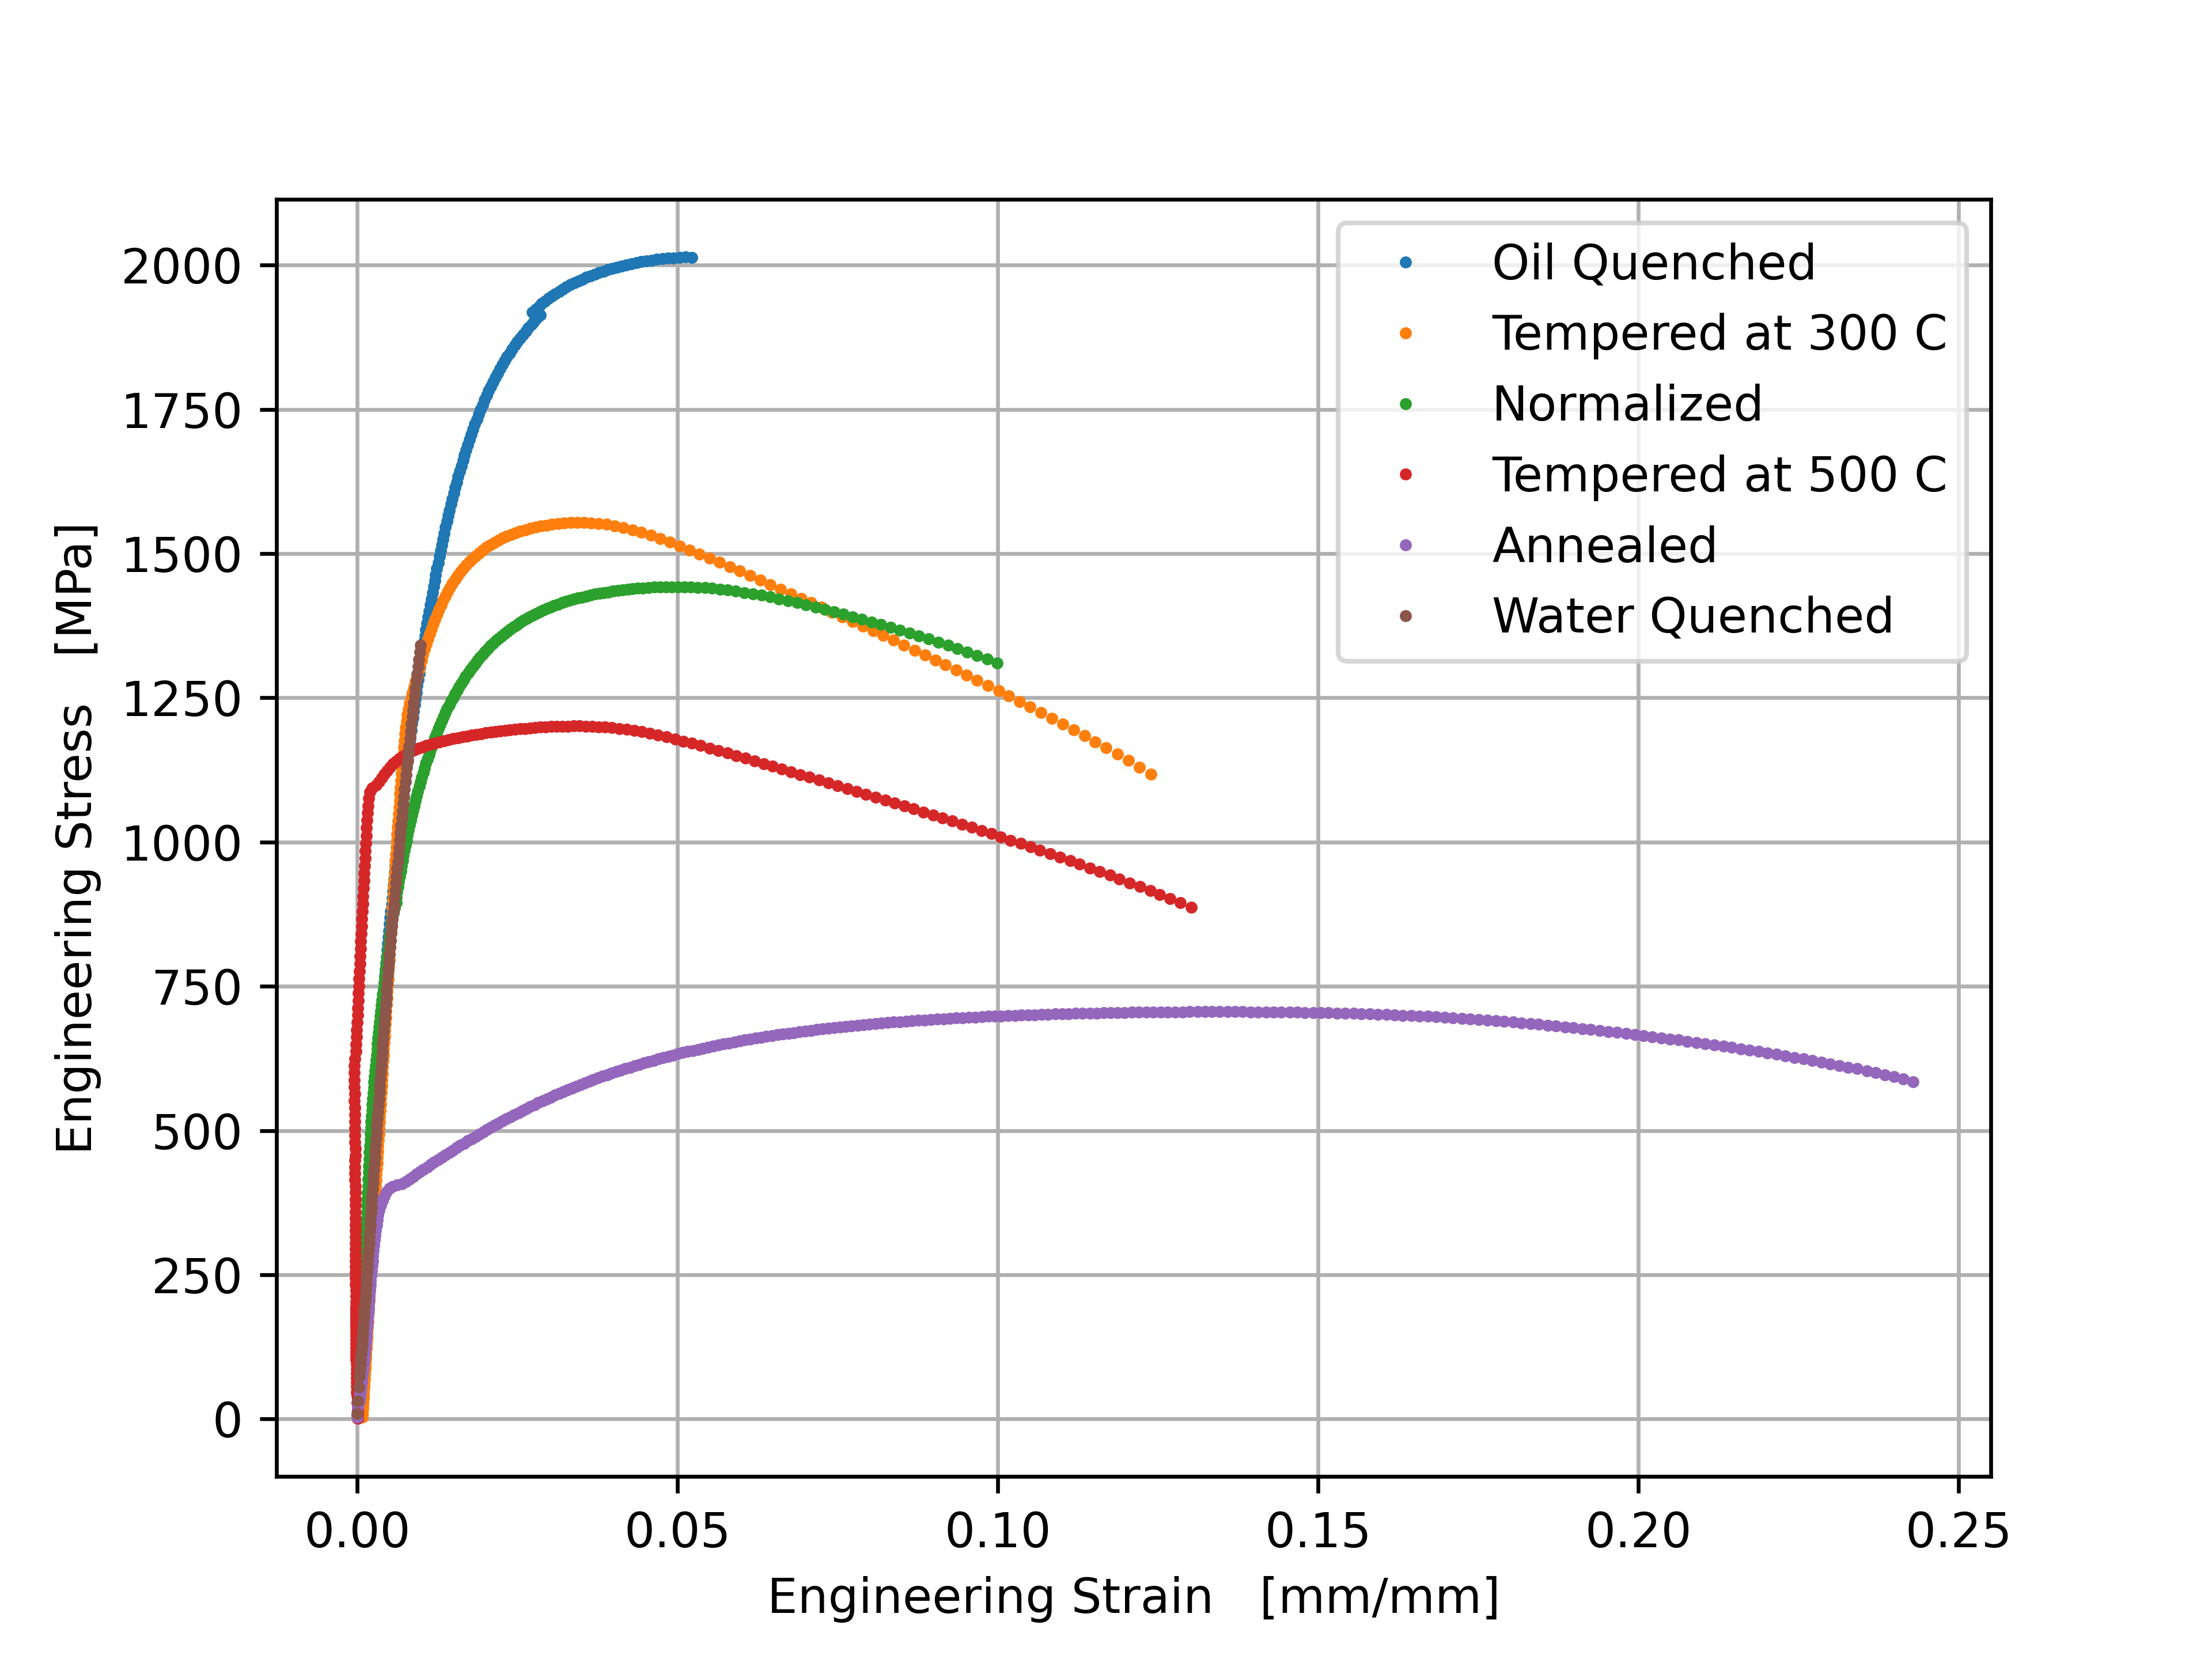
\includegraphics[width=0.5\linewidth]{plots/q1_adjusted.png}
    \caption{Engineering Stress-Strain curves of select materials}
    \label{fig:q1-all}
\end{figure}

Next, from Fig. \ref{fig:q1-all} we found the elastic modulus, the yield strength, the ultimate strength, the toughness, percent elongation, and Brinnel hardness for each specimen. To not have an overly wide table, the specimen names were abbreviated but follow the same order as in the legend of Fig. \ref{fig:q1-all}. The Brinnel hardness values were determined via the conversionary equation, Eq. \ref{eq:rc2br}, from our measured HRC values. The yield strengths were determined via the 0.2 \% offset methodology.

\begin{table}[!h!]
    \centering
    \renewcommand{\arraystretch}{1.5}
    \caption{Select material properties of each specimen tested}
    \begin{tabular}{|c|c|c|c|c|c|c|}
        \toprule
        \hline
        \textbf{Material} & \textbf{OQ} & \textbf{Temp. 300} & \textbf{Norm.} & \textbf{Temp. 500} & \textbf{An.} & \textbf{WQ} \\ 
        \midrule
        \hline 
        \textbf{Youngs Modulus [GPa]} & 197.065 & 186.829 & 205.729 & 227.167 & 111.797 & 161.711 \\ 
        \hline 
        \textbf{Yield Strength} & 1138.428 & 1269.068 & 931.842 & 1148.958 & 402.874 & 1341.104 \\ 
        \hline 
        \textbf{Ultimate Strength} & 2013.803 & 1553.692 & 1442.464 & 1201.172 & 705.882 & 1341.104 \\ 
        \hline 
        \textbf{Toughness} & 86.562 & 166.139 & 131.696 & 142.251 & 155.675 & 7.386 \\ 
        \hline 
        \textbf{Percent Elongation} & 5.22 & 12.392 & 9.992 & 13.061 & 24.284 & 0.991 \\ 
        \hline 
        \textbf{Brinnel Hardness} & 264.692 & 309.453 & 238.109 & 247.905 & 1206.654 & 353.671 \\ 
        \hline 
    \end{tabular}
    \label{tab:q2}
\end{table}

Next, from these tabulated values we can determine a correlation between the  the ultimate strength and Brinnel hardness of each specimen, presented in Fig. \ref{fig:q4}. The linear-regression was performed with the use of \texttt{scipy.stats.linregress}. Next, again from Table \ref{tab:q2}, we determined the correlations between the ultimate strength, the yield strength, the elastic modulus, and the percent of elongation and the Brinnel hardness for specifically the oil quenched and the oil quenched then tempered specimens.

\begin{figure}[!h!]
    \centering
    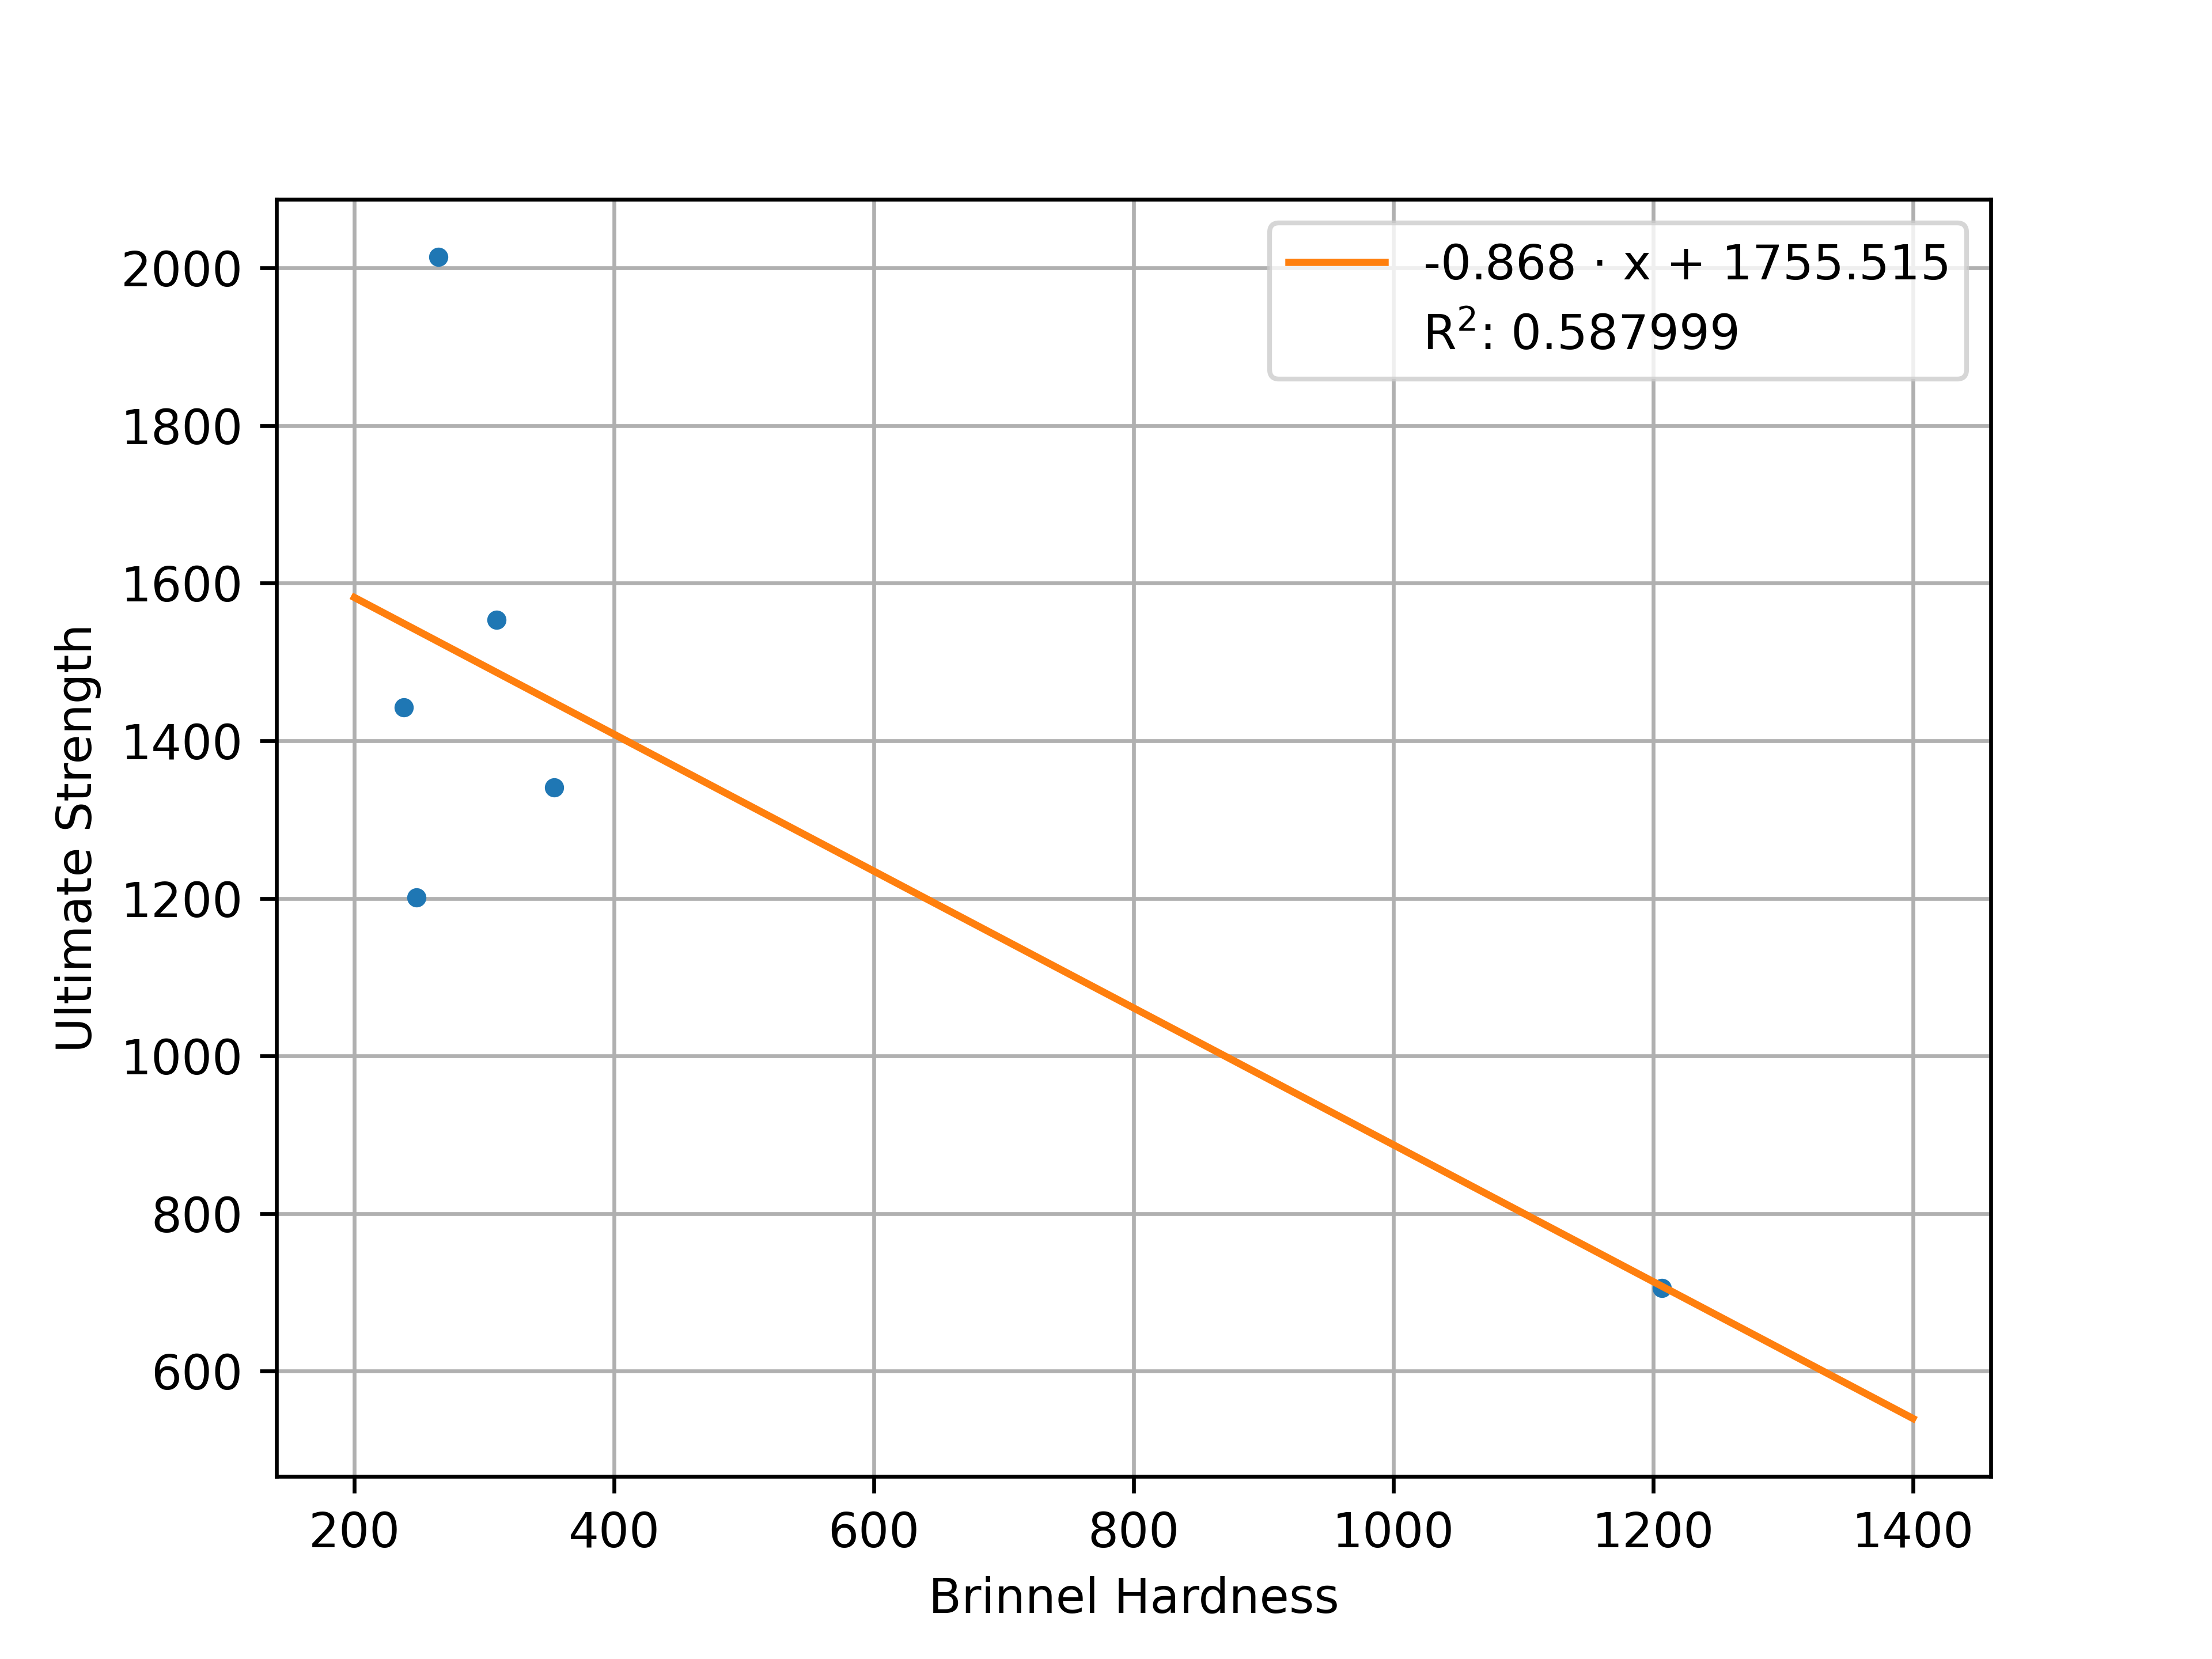
\includegraphics[width=0.5\linewidth]{plots/q4.png}
    \caption{Correlation of $\sigma_{UTS}$ to BHN for all specimens}
    \label{fig:q4}
\end{figure}


\begin{figure}[!h!]
\begin{minipage}[b]{.5\linewidth}
    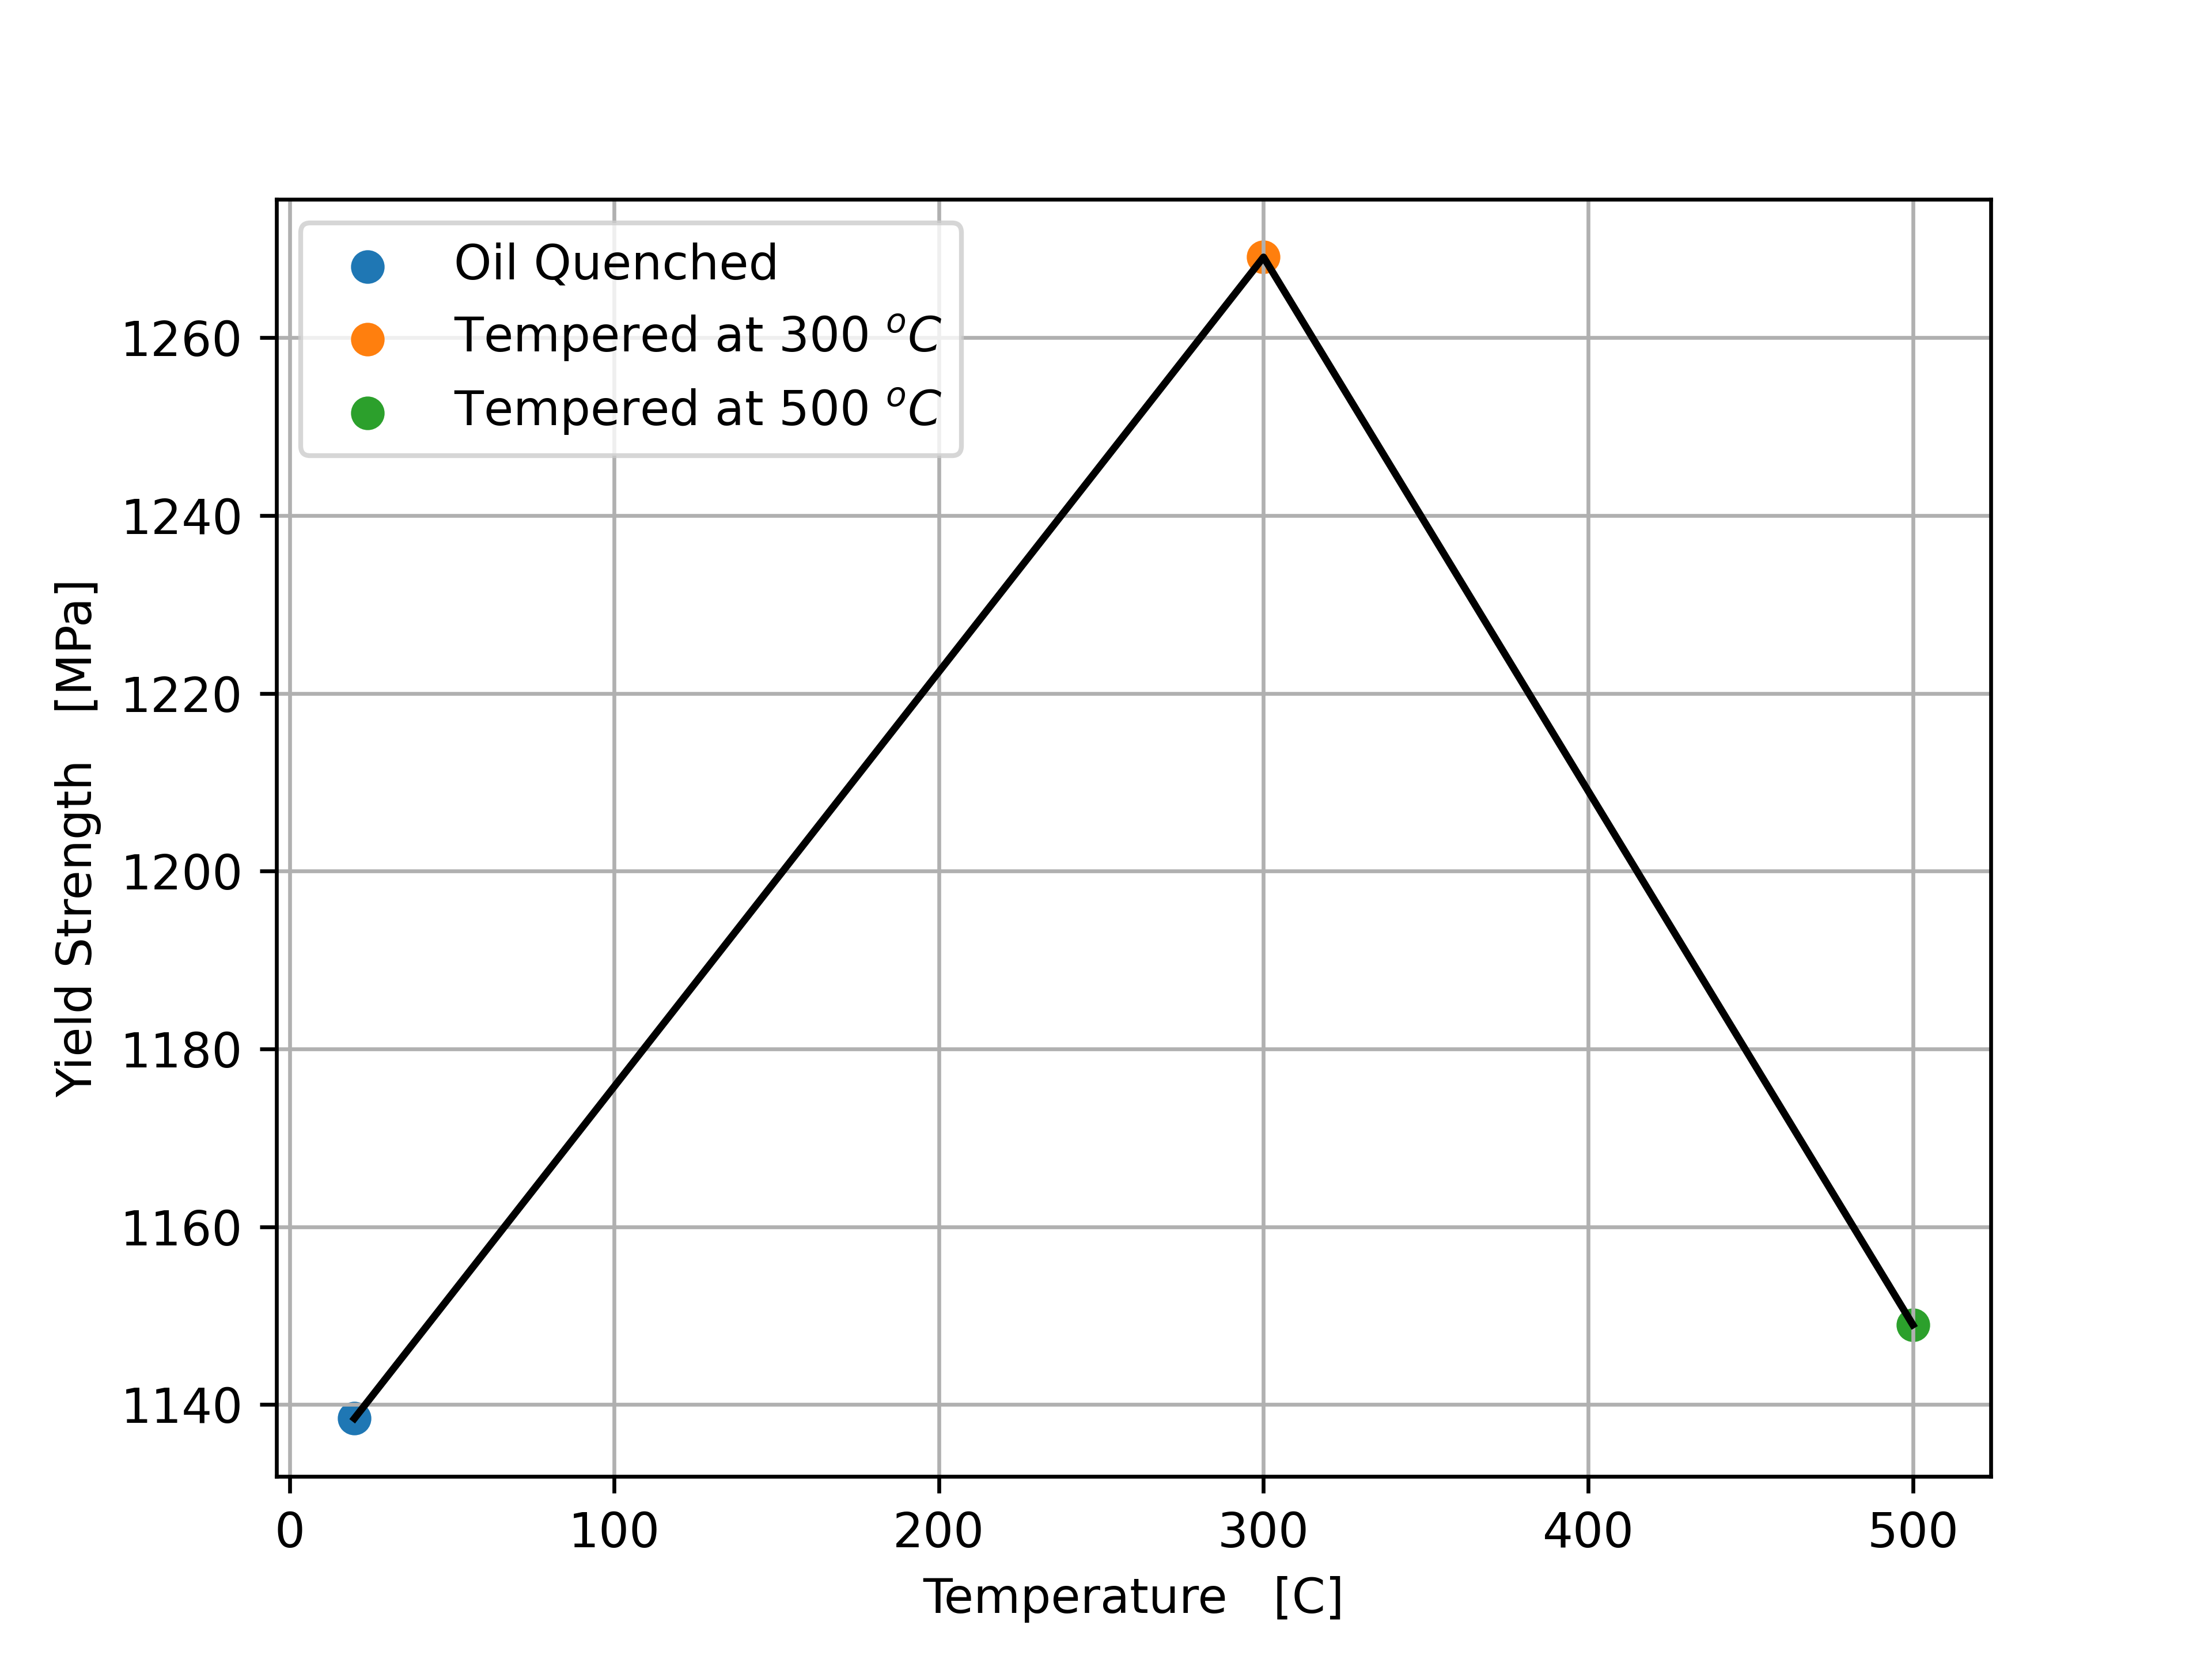
\includegraphics[width=\linewidth]{plots/q6_offset.png}
    \caption{Correlation of $\sigma_y$ to BHN}
    \label{fig:q6-yield}
    \vspace{4ex}
\end{minipage}
\begin{minipage}[b]{.5\linewidth}
    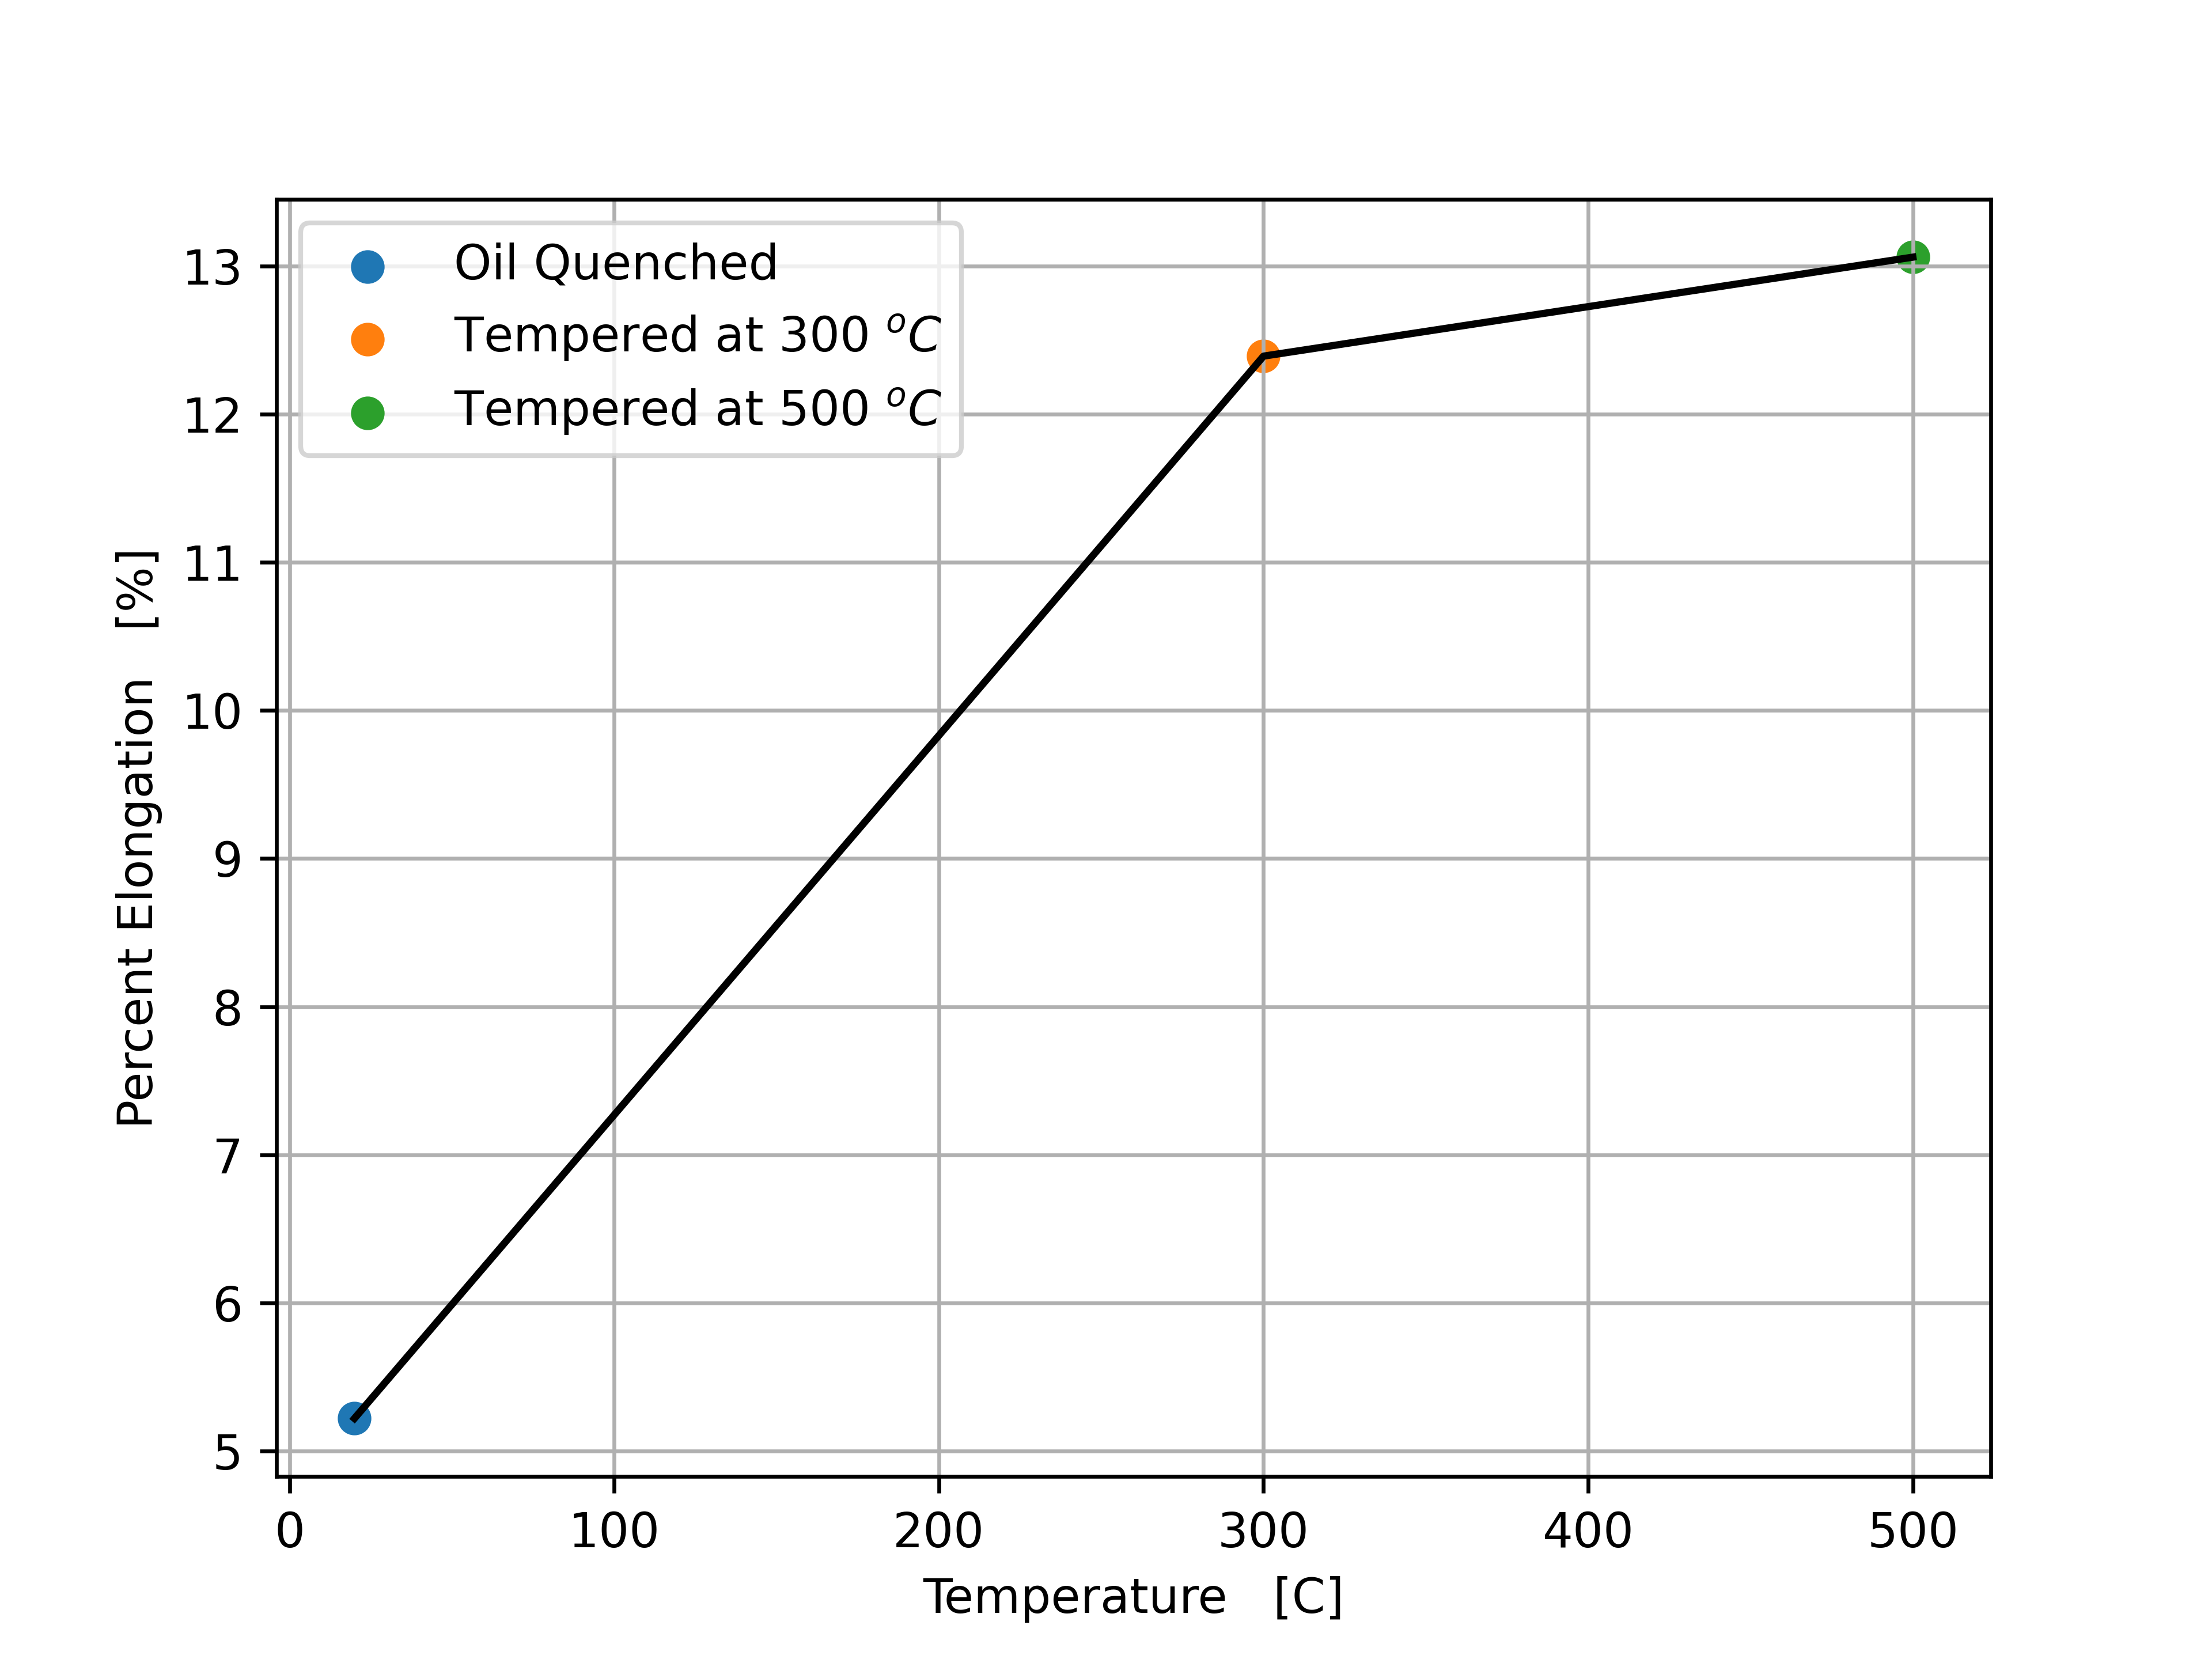
\includegraphics[width=\linewidth]{plots/q6_per_elong.png}
    \caption{Correlation of $\%_{elongation}$ to BHN}
    \label{fig:q6-perelong}
    \vspace{4ex}
\end{minipage}
\begin{minipage}[b]{.5\linewidth}
    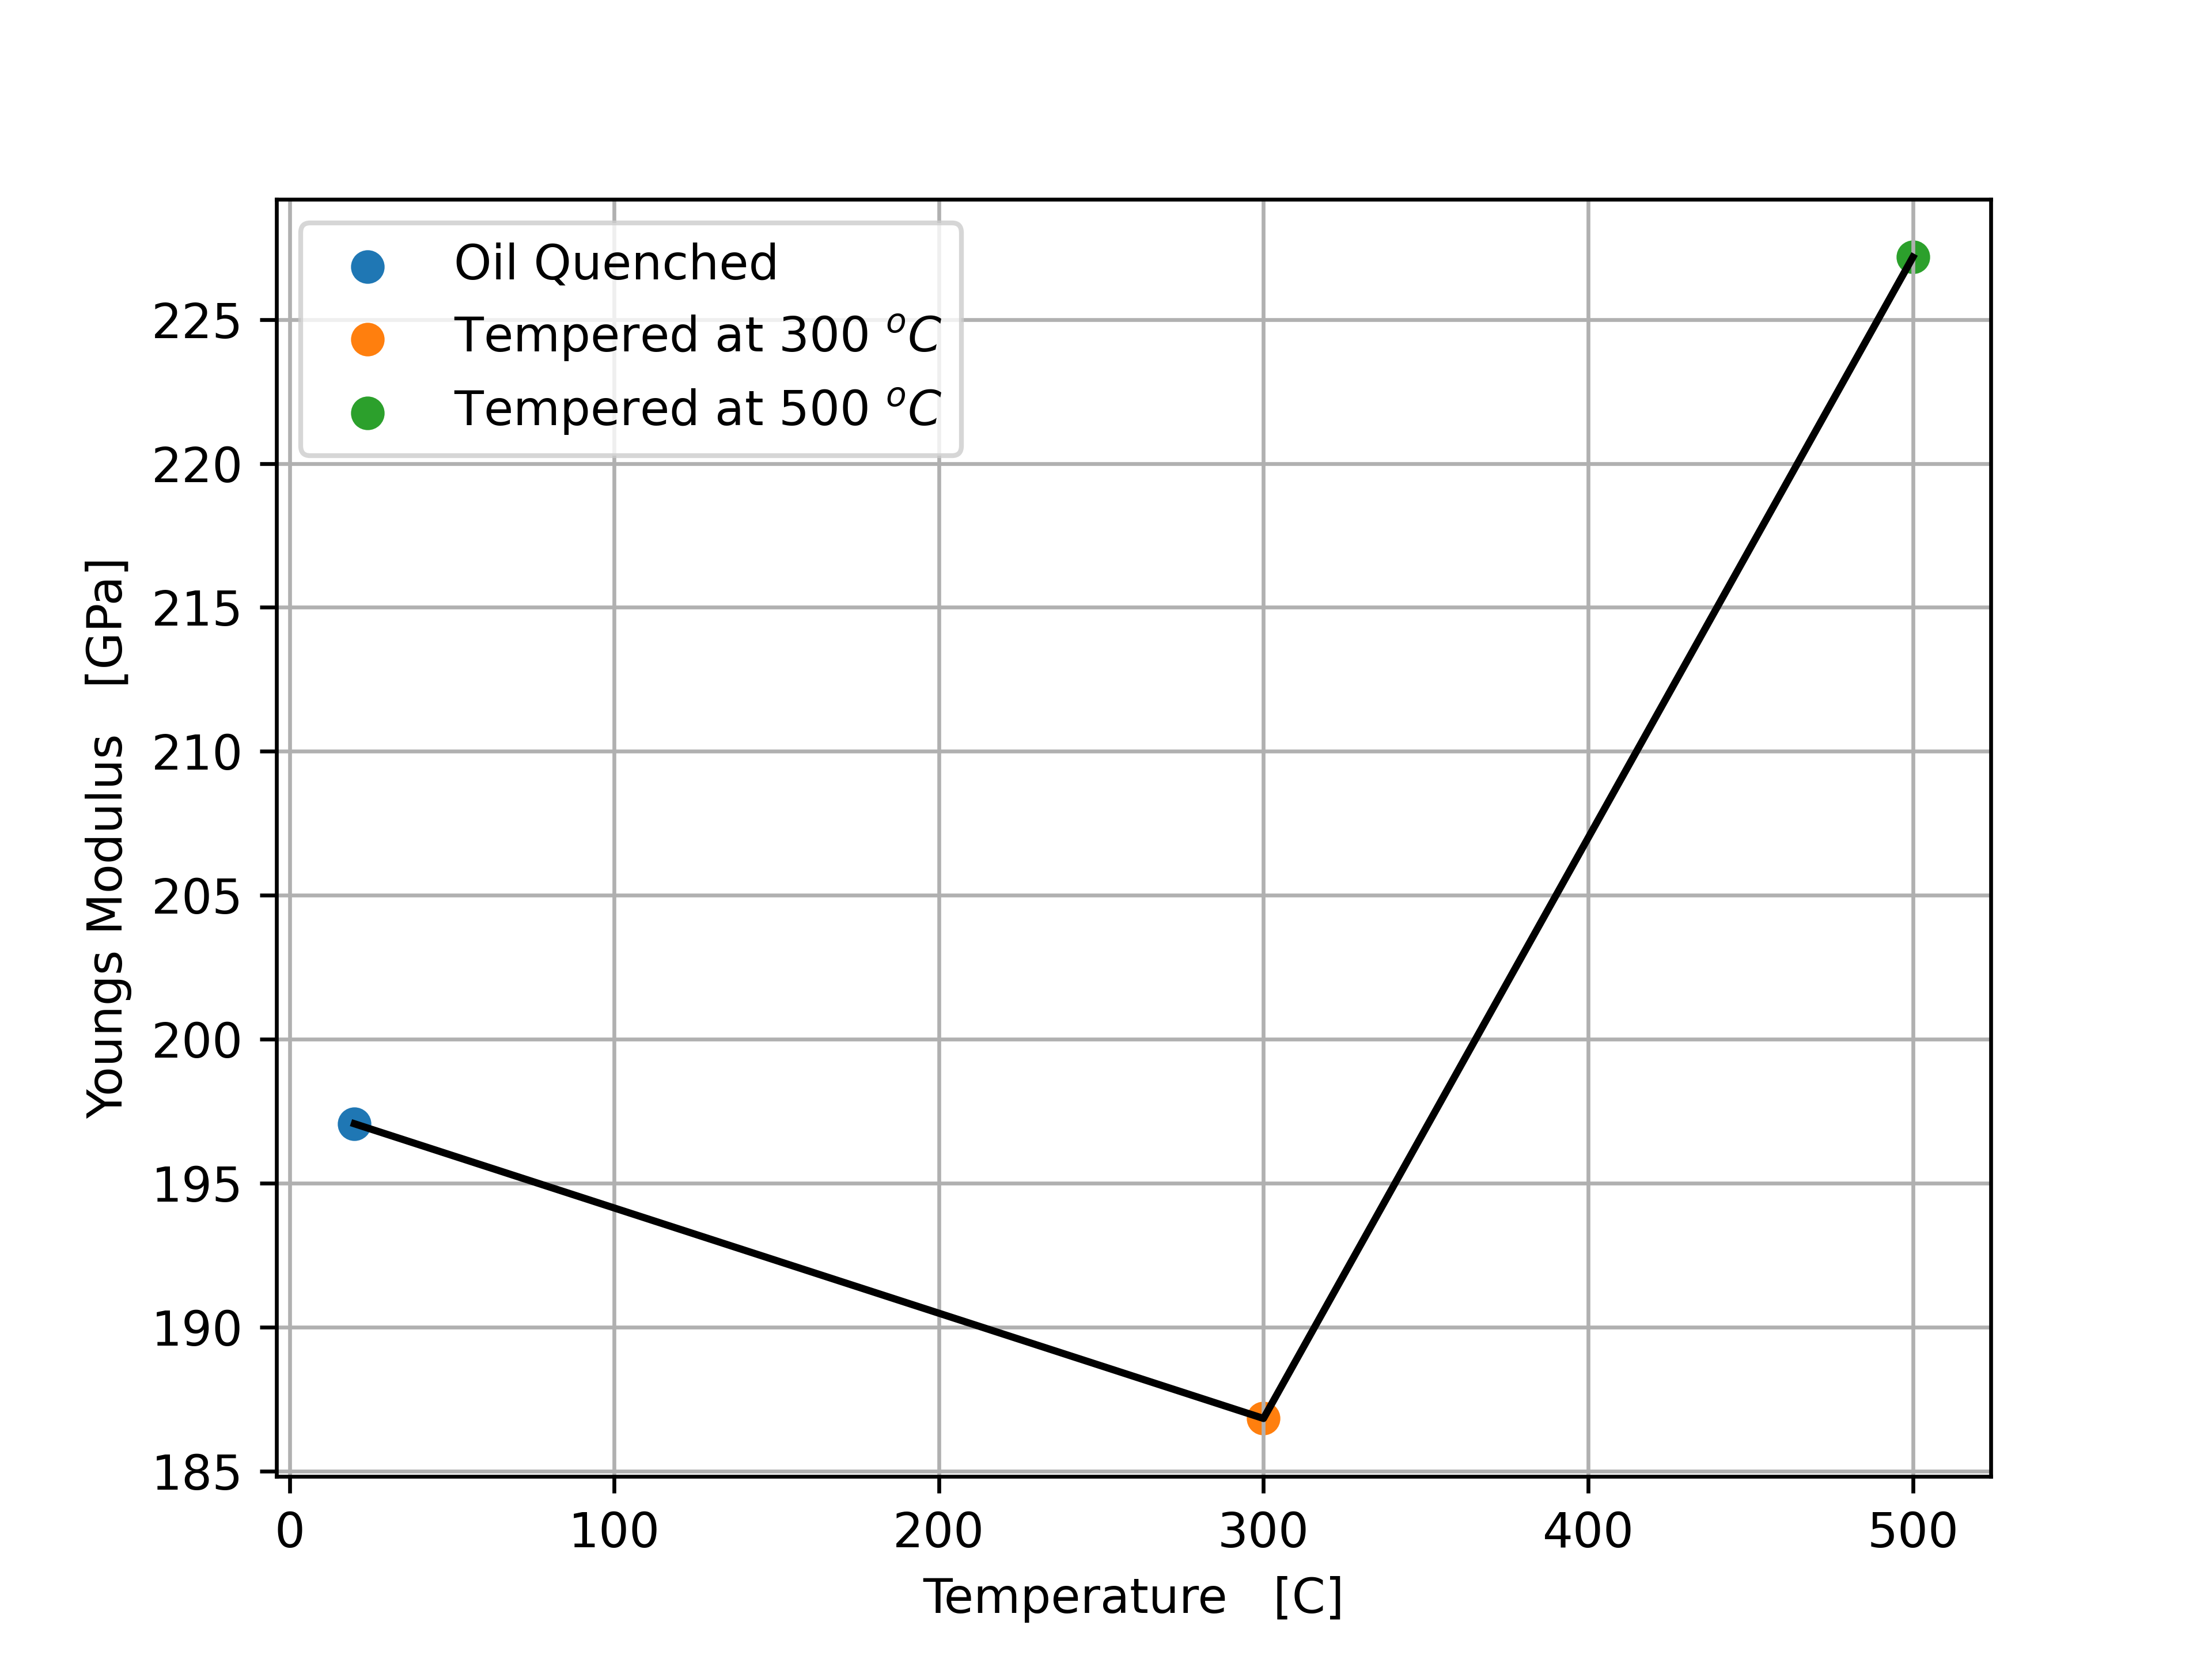
\includegraphics[width=\linewidth]{plots/q6_youngs.png}
    \caption{Correlation of $E$ to BHN}
    \label{fig:q6-youngs}
    \vspace{4ex}
\end{minipage}
\begin{minipage}[b]{.5\linewidth}
    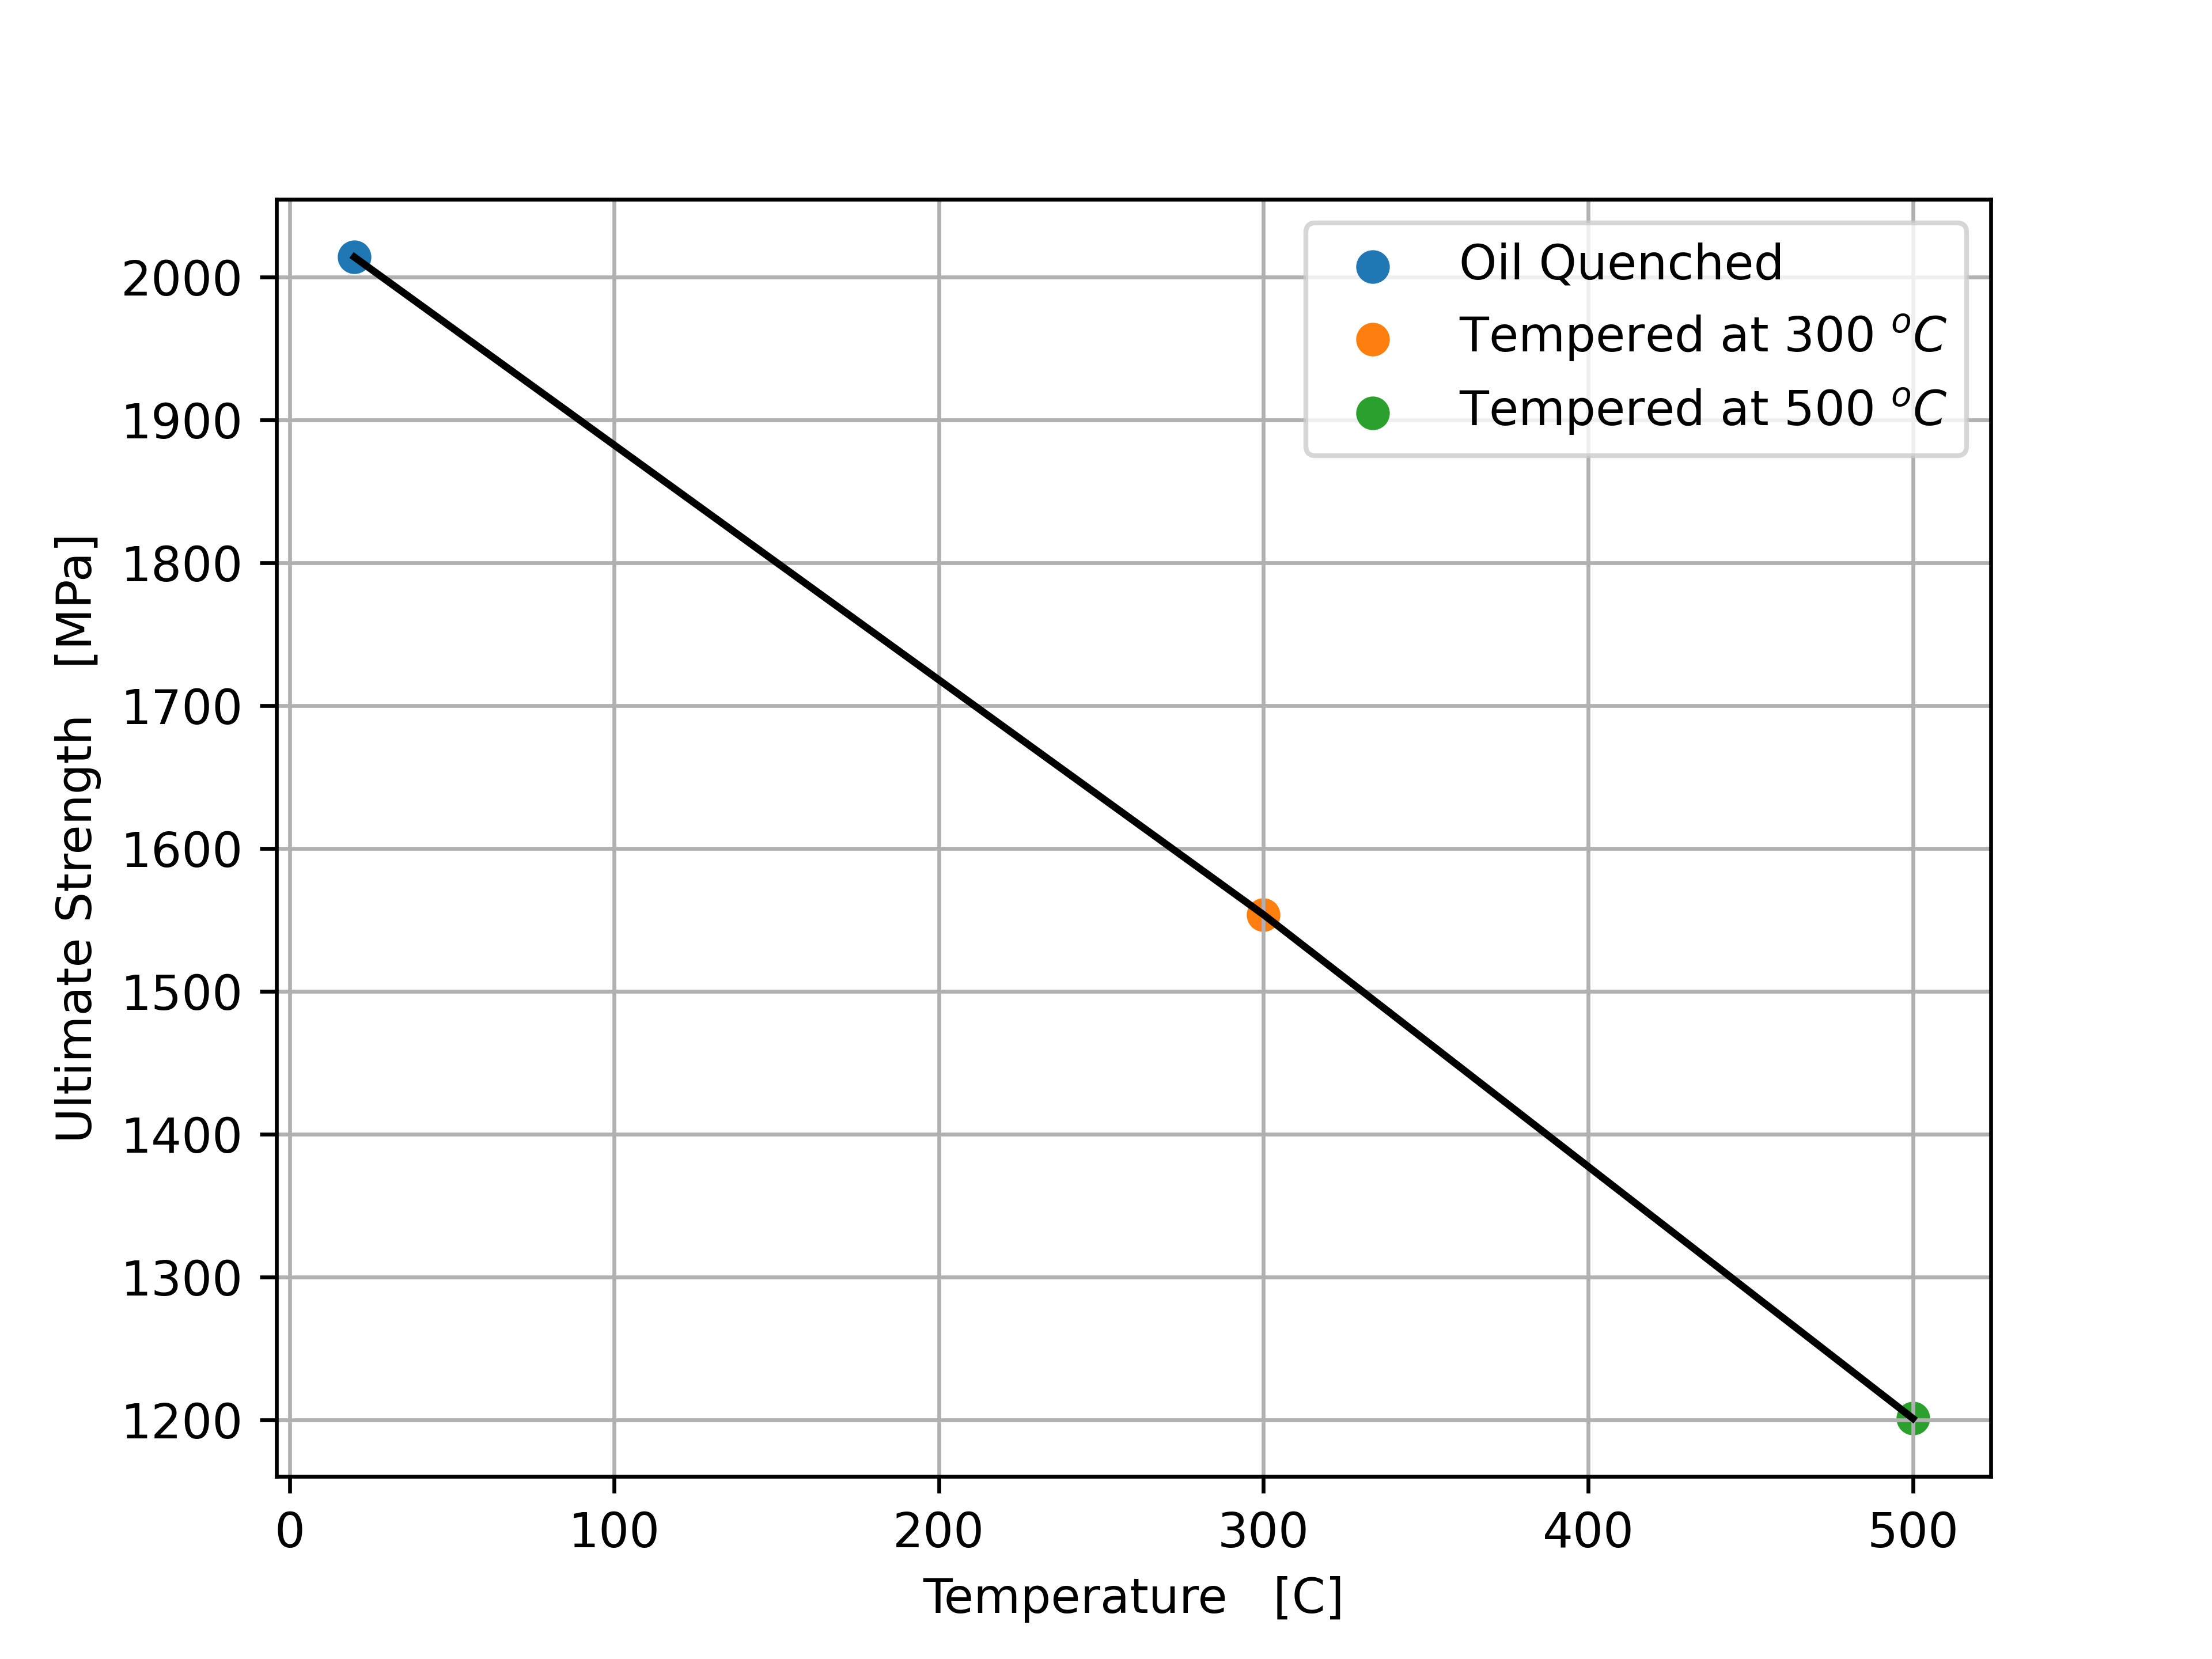
\includegraphics[width=\linewidth]{plots/q6_uts.png}
    \caption{Correlation of $\sigma_{UTS}$ to BHN}
    \label{fig:q6-uts}
    \vspace{4ex}
\end{minipage}
\end{figure}
\newpage

\section{Analysis of Discussion and Results}
To begin, our true-uncorrected data is rather lugubrious. This is due to mal-practice in loading of specimens, and so many of our trials either began with negative strains or started at 0 and then went negative prior to going positive. To amend these poor results, we chopped off the objectively incorrect data points that were obviously produced from incorrect loading, and then performed our data processing on the resulting datasets. For example, our normalized stress strain curve:

\begin{figure}[!h!]
    \centering
    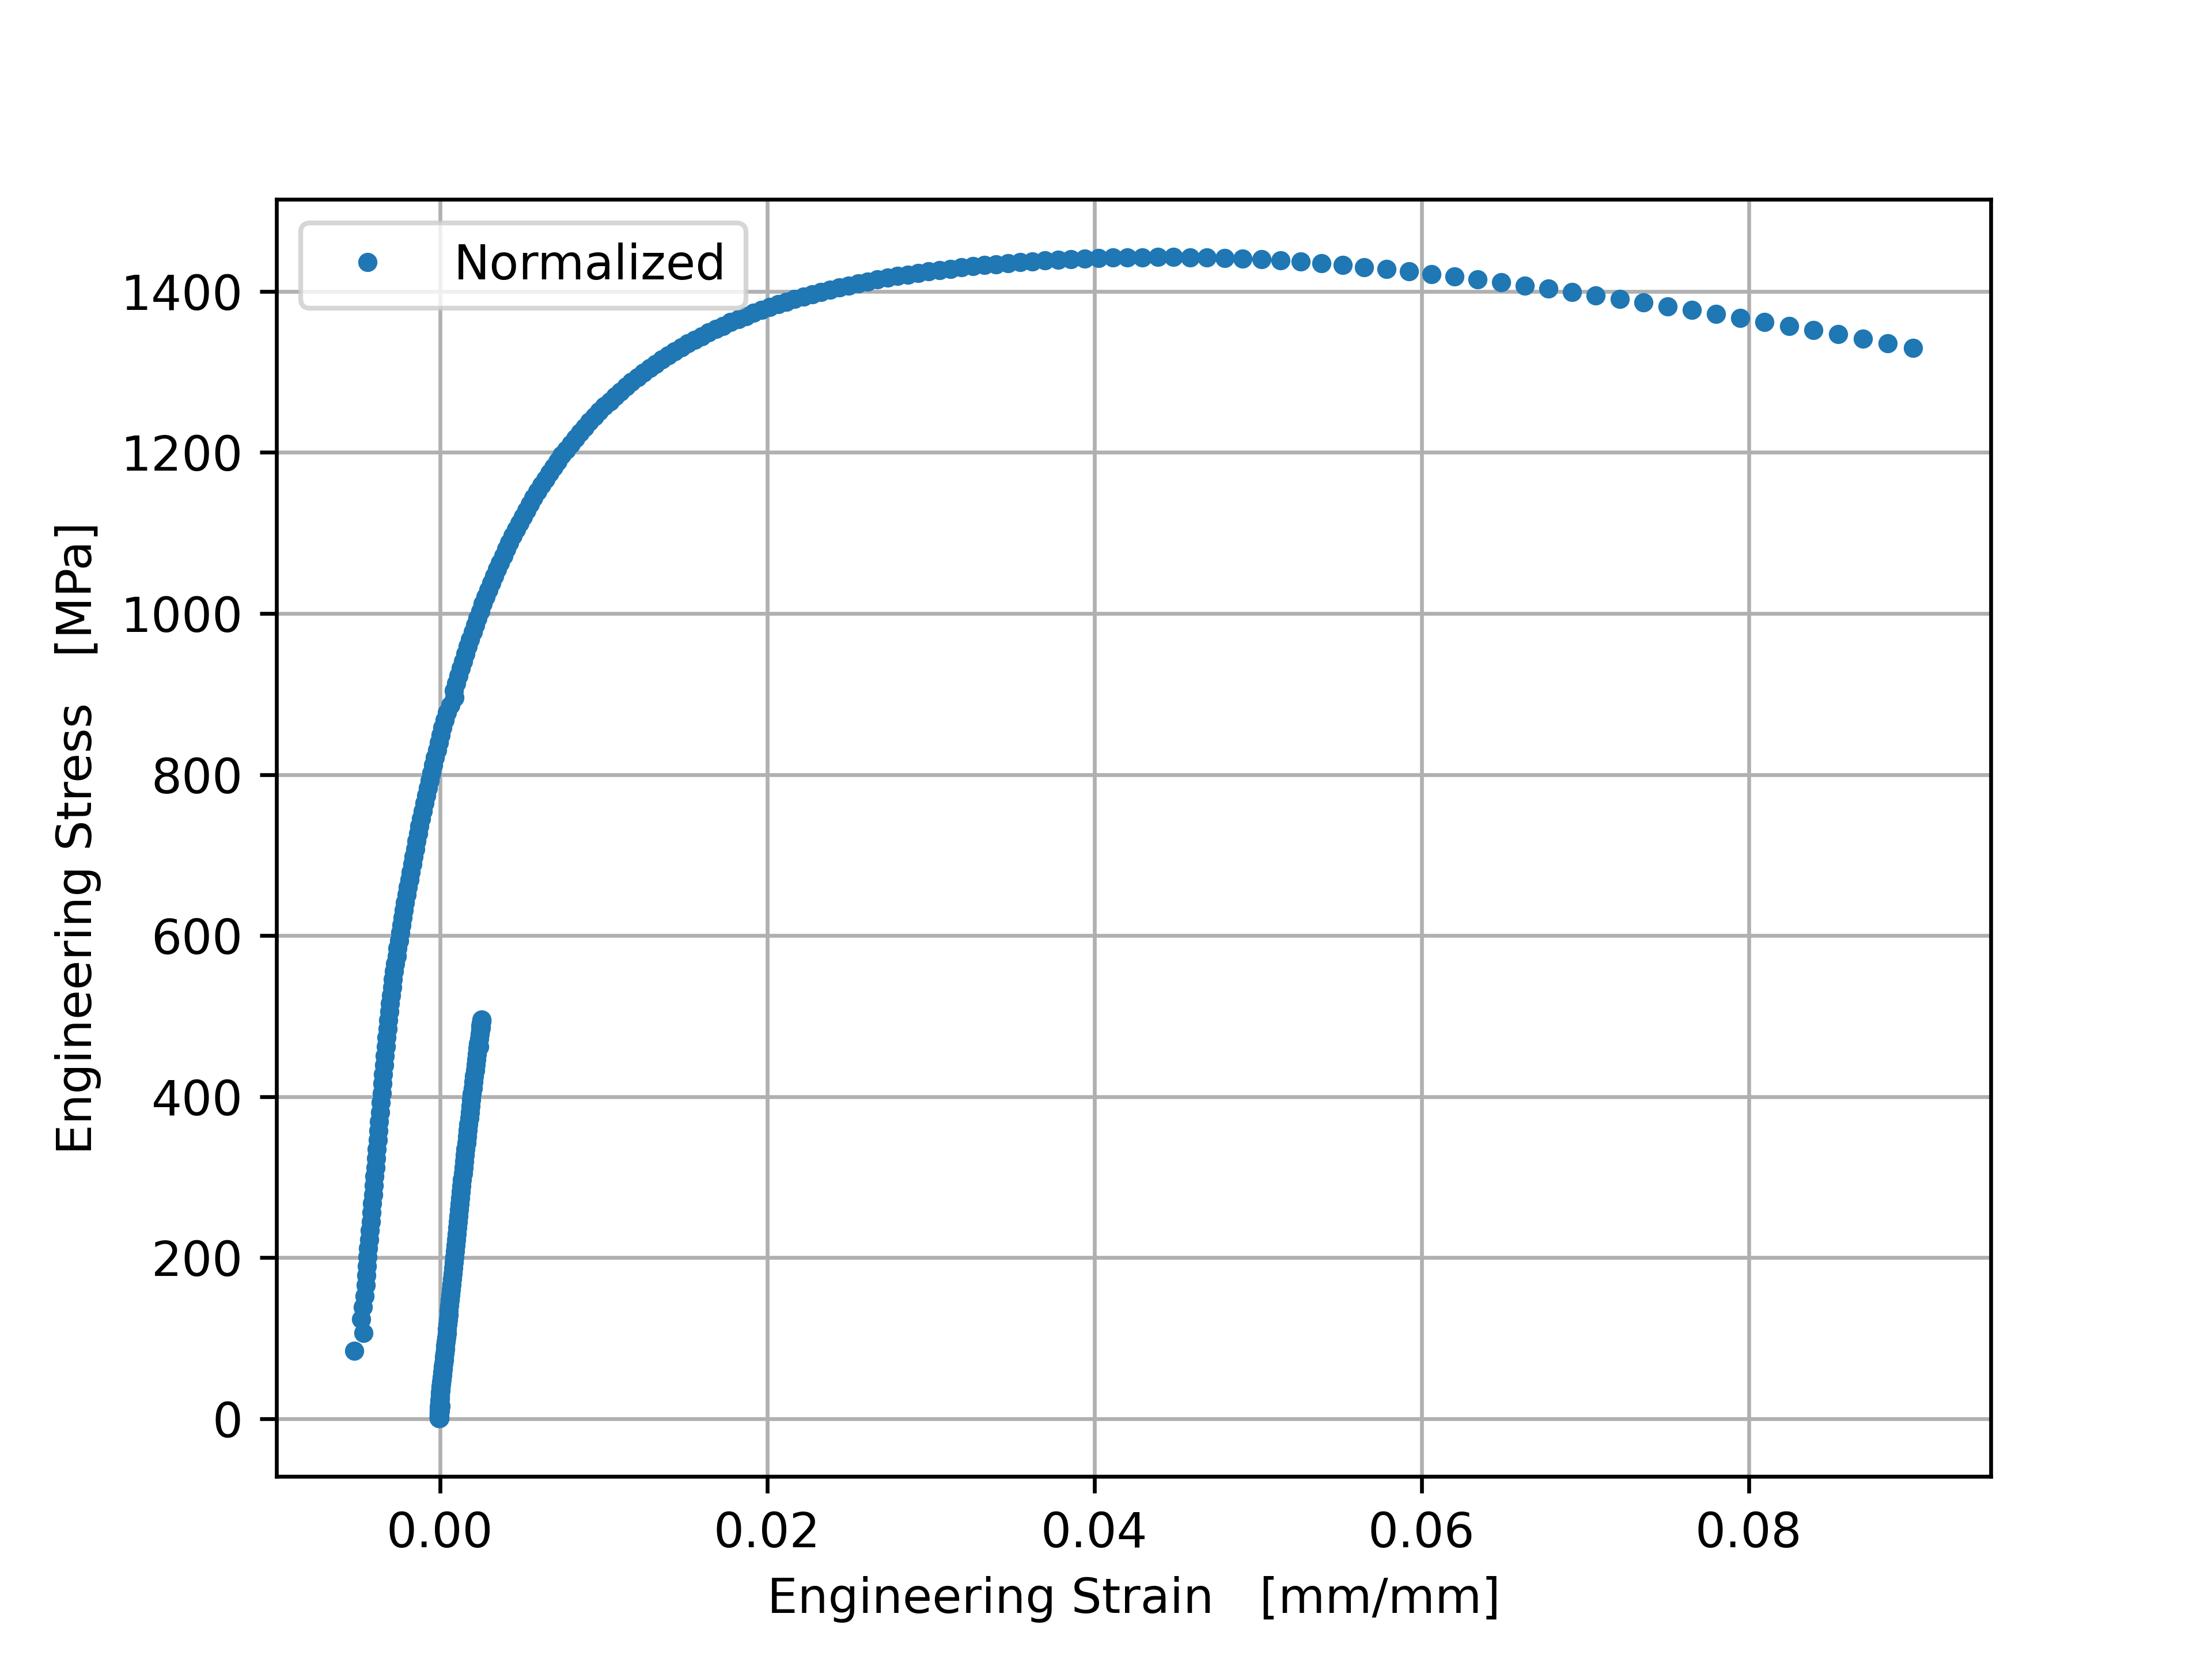
\includegraphics[width=0.5\linewidth]{plots/bs_plot.png}
    \caption{Normalized Stress-Strain curve, pre-adjusting}
    \label{fig:bs-plot}
\end{figure}

To fix this data set, we chopped the initial loading phase from the data set, removing the strong discontinuity. 

To continue, another strong source of error was in finding the Brinnel hardness of the annealed sample. This is due to the invalidity of application of the equation we utilized to convert between Rockwell C and Brinnel for this specimen. Similarly, when determining the toughness of the water quenched sample, because our mechanism in determining yield strength resulted in equivalent fracture point and yield strengths, the numerical integration was invalid. To obtain a non-zero value we integrated from 0 to the fracture point. We recognize this is invalid. 


\newpage
\section{Answer to Questions}
\subsection*{Question 1}
To begin, we found and plotted the engineering stress-strain curves of various heat treatment methods enacted upon 4340 specimens. We investigated basic water quenched, basic oil quenched, annealed, normalized, oil quenched then tempered at 300 $^oC$, and oil quenched then tempered at 500 $^oC$. These curves are presented in Fig. \ref{fig:q1-all}.

\subsection*{Question 2}
Next, we found the elastic modulus, yield strength, ultimate tensile strength, toughness, percent elongation, and brinnel hardness of each aforementioned specimen. These values are tabulated in Tab. \ref{tab:q2}. Various results stand out, namely the yield strength of the water quenched specimen and the hardness of the annealed specimen. For the water quenched specimen, unfortunately when utilizing the 0.2\% offset method to determine the yield strength, the offset linear line never intercepted with the stress-strain curve as the specimen failed prior to significant plastic deformation. Further, the Brinnel hardness value for the Annealed specimen is absurdly high. This is due to the Rockwell hardness being very large ---- 87.9 ---- and outside of the range of validity of our empirically derived conversion equation, Eq. \ref{eq:rc2br}.

\subsection*{Question 3}
Noticeably, the material properties for each specimen are starkly different despite all being 4340. This is due to the affect that heating and cooling have on the microstructure of materials. In 4340, the faster the specimen is cooled the more martensite is present, and the more brittle the specimen is. The strongest specimen, by far, was the standard oil quenched specimen. The hardest was the annealed specimen. The stiffest was the water quenched whereas the most ductile was the annealed specimen. Finally, the toughest was the oil quenched then tempered at 300 $^oC$.

\subsection*{Question 4}
We determined the relationship between the ultimate tensile strength and the Brinnel hardness of each specimen, presented in Fig. \ref{fig:q4}. Our linear regression yielded a less than optimal correlation ---- only 0.588. Despite the poor fit, we do expect an inverse relationship between hardness and ultimate strength. We expect this as the harder a material is, the tougher we expect, and thus the less ductile. This is a gross over-simplification on the relationship between hardness and strength, but is sufficient for comparison's sake. 

\subsection*{Question 5}
The heat treatment that results in potential surface flaws is water quenching. This is due to the rapidity in cooling due to the high thermal conductivity of water. This rapid cooling is so strong and fast that it exerts huge thermal stresses upon the specimen, where portions of the surface experience rapid thermal de-expansion, potentially yielding cracks that can propagate through the material during tensile load. In fact, this was present in our water quenched specimen, where the specimen failed prior to non-negligible plastic deformation. 

\subsection*{Question 6}
Next, we determined the relationships between ultimate strength, yield strength, elastic modulus, and percent elongation versus tempering temperature for all of the oil quenched specimens. These specimens are the simple oil quenched, the oil quenched then tempered at 300 $^oC$, and the oil quenched then tempered at 500 $^oC$. These relationships are presented in Figs. \ref{fig:q6-yield} - \ref{fig:q6-uts}.


\subsection*{Question 7}
To begin to compare the microstructure of three cooling methods, the microstructure are presented below. Fig. \ref{fig:an} is the annealed specimen, thus the small dark globules are pearlite, and the smaller circular globules are spherodite. Fig. \ref{fig:wq} is the water quenched specimen, and the vast majority of the structure is martensite. Finally, Fig. \ref{fig:nm} is the normalized specimen, where the dark globules are pearlite and the light globules are ferrite. To compare these microstructures, we will analyze the resulting material properties. Firstly, martensite will have relatively poor ductility, due to the high dislocation density from a large quantity of grain boundaries. On the contrary, the annealed specimen has high uniformity and thus low relative dislocation density and high ductility. in the middle however reside the normalized specimen, where there is a high quantity of two different phases, but low mixing. Because of this combination, the normalized steel will have better ductility than the water quenched, but worse than the annealed; and conversely more strength than the annealed but less than the water quenched.  
\newpage
\begin{figure}[!h!]
    \centering
    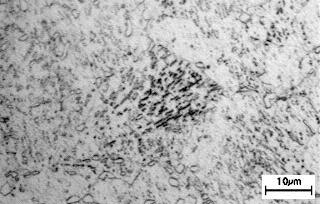
\includegraphics[width=0.5\linewidth]{plots/microA.jpg}
    \caption{Annealed Specimen}
    \label{fig:an}
\end{figure}
\begin{figure}[!h!]
    \centering
    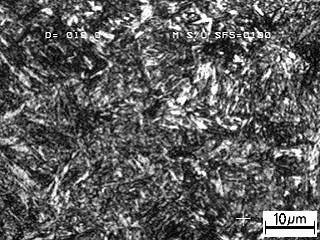
\includegraphics[width=0.5\linewidth]{plots/microB.jpg}
    \caption{Water Quenched Specimen}
    \label{fig:wq}
\end{figure}
\begin{figure}[!h!]
    \centering
    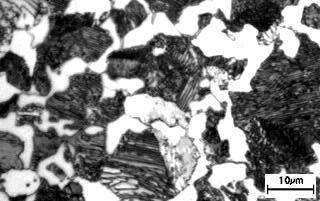
\includegraphics[width=0.5\linewidth]{plots/microC.jpg}
    \caption{Normalized Specimen}
    \label{fig:nm}
\end{figure}

\newpage
\subsection*{Question 8}
To begin, for the Annealed specimen we can see the formation of both pearlite and spherodite. Due to the prominence of the spherodite phase, we can assume the specimen austenitized. To satisfy all of these conditions the steel must be between 0.77\% and 4.3\% carbon, and additionally due to the strong prominence of spherodite we can assume the carbon content is higher than 2.1\% carbon. Next, the normalized specimen. We observe prominence of both ferrite and pearlite. Due to the presence of ferrite, the carbon content must be below .83\% carbon, however due to the strong prominence of this phase there must be more than 0.5\% carbon. Finally, the water quenched specimen. This specimen is entirely martensite, and thus must be between 0.2\% and 0.65\% carbon content \cite{lab5paper}. 



\subsection*{Question 9}
Different microstructures arise from varying heat treatments because the formation of grains and their size are strongly dependent on the rate of thermal energy removal from the specimen. This is due to dislocations, such as grain boundaries, being structural defects and, given enough energy, can rectify themselves. Excess thermal energy being supplied to the system increases the rate in which these defects rectify themselves, and thus one could presume that slowly cooling a specimen or holding a specimen at a high solid temperature would result in a low dislocation density (low quantity of grains), and conversely rapid cooling yields large quantities of grains and dislocations. The material properties of steel are partially a result of the structure of a perfectly mixed steel sample aswell as the dislocations interacting with each other and external forces. For example, the higher the dislocation density normal to the direction of applied load, the more resistive the material will be to that load. This is simply due to the sheer number of shearing forces needed to cause slip. 
\newpage

\section{Conclusions}
In conclusion, we found a strong causality correlation between material properties and heat treatment method utilized, often yielding drastically different properties. We found quicker cooling treatments yielded stronger materials that were more brittle, and slower treatments or treatments that were held at an elevated temperature to have much more ductility at the cost of a lower strength. Finally, we identified the causality for the difference between material properties to be the specific phase of the microstructures in the specimens, where martensite lead to poor ductility and spherodite and pearlite lead to more ductility.

\section{Bibliography}
\printbibliography[heading=none]
\end{document}